\documentclass[letterpaper,11pt]{article}
\author{Ashley Towne\\Advisor: A. P. Hickman}
\title{Semiclassical Analysis of Quantum Mechanical Calculations of Rotationally Inelastic Collisions of He and Ar with NaK$^\dagger$}
\pagestyle{plain}
\usepackage{graphicx}
\usepackage{subcaption}
\usepackage{amsmath}
\usepackage{epstopdf}
\bibliographystyle{mysty}
\newcommand{\vectorize}[1]{\boldsymbol{#1}}

\begin{document}
\maketitle
\begin{center}
    \abstract{Recent quantum mechanical calculations and laboratory experiments
        at Lehigh University have provided detailed information about
        rotationally inelastic collisions of He and Ar with NaK in a cell at
        thermal energies.  The purpose of this project was to develop a
        semiclassical model for these collisions based on the well-known vector
        model.  In the quantum mechanical theory, Grawert coefficients
        $B_\lambda(j,j')$ (where $\lambda$ is an integer) give the probability
        that a discrete amount $\lambda \hbar$ of angular momentum is
        transferred from the projectile to the target in a transition between
        rotational levels $j$ and $j'$.  Derouard showed that one can develop a
        semiclassical model by transforming from $\lambda$ to the continuous
        variable $\alpha$, the angle between initial and final angular momentum
        vectors $\vectorize{j}$ and $\vectorize{j'}$.  In the present work we
        invoked the vector model, which relates the polar angle $\theta$ of the
        angular momentum vector to the azimuthal quantum number $m$, and showed
        that the distribution $P(\theta,\theta')\sin\theta'$ of final polar
        angles $\theta'$ could be expressed as a convolution of the
        semiclassical Grawert coefficient $B(j,j';\cos\alpha$).  Using this
        expression we calculated the expected distribution of values of $\Delta
        \theta = \theta' - \theta$ and compared it with the quantum mechanical
        result.  The semiclassical model agreed very well with the quantum
        mechanical theory, especially when the quantum number $j$ was large.
        The distribution of projections of $j$ onto the $z$ axis before and
        after collision (in a transition $jm \rightarrow j'm'$) demonstrated
        (as others have also noticed) that $m$ changes in such a way that
        $\theta$ tends to be preserved. The semiclassical model also predicts
        the propensity for collision-induced changes in $j$ to be even numbers,
    in agreement with quantum mechanical theory and experiment.}

    \vspace{2pt}
    \noindent{$^\dagger$\small{Work supported by NSF grants PHY-1359195, PHY-0968898, and PHY-1403060.}}

\end{center}

\clearpage
\tableofcontents
\clearpage
\section{Introduction}
NaK, like any molecule, can vibrate and rotate and can be described by the
quantum numbers that characterize these vibrational and rotational states.
Upon collision with a perturbing atom, such as helium or argon, these quantum
numbers can change, signifying a transition from one state to another.  This
project is primarily concerned with collisions where the vibrational state is
conserved, but the rotational state changes, as Eq.~\ref{eq:collisions}
specifies.  
\begin{eqnarray}
    \mathrm{He}+\mathrm{NaK}(v,j,m)&\rightarrow& \mathrm{He}+\mathrm{NaK}(v,j',m') \nonumber\\
    \mathrm{Ar}+\mathrm{NaK}(v,j,m)&\rightarrow& \mathrm{Ar}+\mathrm{NaK}(v,j',m') \nonumber\\
    \label{eq:collisions}
\end{eqnarray}
Specifically, the purpose of this investigation was to explore the physical
interpretation of how the quantum numbers that describe angular momentum
change during collision.  The vector model was extended to describe not only
one angular momentum state but a transition between two states.

In addition to its rotational and vibrational states, NaK can also be described
by its electronic state, which the set of potential curves express. A set of
NaK's potential curves, calculated by Magnier~\cite{Mag00}, can be seen in
Figure~\ref{fig:potentialcurves}. The potential curves represent energy as a
function of internuclear separation between sodium and potassium. Both
experimental and theoretical investigations choose one potential curve to
study, specifying the electronic energy level at which the collisions in
question take place.
\begin{figure}[ht]
    \centering
    \includegraphics[width=0.6\textwidth]{potentialcurves.eps}
    \caption{Potential curves for NaK. The electronic state of interest for this work is the first excited $^1\Sigma^+$ state.}
\label{fig:potentialcurves}
\end{figure}

\section{Background}
\subsection{Experimental Measurements}
At Lehigh University, the experimental and theoretical groups have worked
together to investigate the collisions in question.  Recent experiments have
studied NaK+He, NaK+Ar, NaK+K, NaCs+He, and NaCs+Ar
collisions~\cite{Jon15,Wol11}.  Related theory has examined NaK+He and NaK+Ar
collisions as well as trends in the vector model and its semiclassical
approximations in~\cite{Mal15,Ale83,Der84}.  Currently at Lehigh, Professor
Huennekens leads the experimental group, and Professor Hickman leads the theory
group.

Professor Huennekens' group has measured the rate constants $k$ of transitions,
which are related to the cross sections~\cite{Hue15}.  The rate
constants are proportional to the thermal average of the product of the cross
section and velocity, which can be approximated as the cross sections times the
average velocity:
\begin{equation}
    k=\langle\sigma v\rangle
\label{eq:rate_constants}
\end{equation}
The cross section is proportional to the likelihood that a particular transition
will occur from one $j$ state to another.  The rate constants average over all
values of the quantum number $m$.

The experimental group has also measured the fraction of orientation that is
preserved throughout the collisions~\cite{Hue15}.  Collisions tend
to be randomizing processes, so studying the extent to which orientation is
preserved gives information about the extend to which a collision changes the
direction of the angular momentum vector. In a cell environment, such as the system that
the experimental group studies, the angular momenta initially point in all
directions and the average value of $m$, or $\langle m\rangle$ is zero; in
other words, the orientation is zero.  In order to measure the change in
orientation, the initial orientation must be nonzero.  The orientation is
proportional to the expectation value of $m$ for a particular $j$ state:
\begin{equation}
    O^j=\frac{\langle m\rangle}{\sqrt{j(j+1)}}
    \label{eq:orientation}
\end{equation}
Physically, it is the extent to which all angular momenta are oriented, or
point in the same direction.

\subsection{Vector Model}
The orientation is  related to the geometric relationship between $m$ and $\vectorize{j}$
in the vector model.  The vector model provides a way of understanding angular
momentum, where $\vectorize{j}$ is the angular momentum vector, and what it means for all
angular momenta to point in the same direction.  As seen in
Figure~\ref{fig:vectormodel}, the quantum number $m$ is the projection of $\vectorize{j}$
onto the $z$ axis:
\begin{figure}[ht]
    \centering
    \includegraphics[width=0.35\textwidth]{vectormodel.eps}
    \caption{Vector model of angular momentum}
\label{fig:vectormodel}
\end{figure}
$\vectorize{j}$ can precess around the $z$ axis at a constant $\theta$ without changing its
magnitude or the magnitude of $m$, as stated by
Eq.~\ref{eq:vector_model_geometry}:
\begin{equation}
    \cos\theta=\frac{m}{\sqrt{j(j+1)}}
    \label{eq:vector_model_geometry}
\end{equation}
The expectation value of the $\cos\theta$ is the orientation, as
Eq.~\ref{eq:orientation} stated.

\subsection{Experimental Procedure}
In order to ensure a nonzero orientation for the initial state of the system,
the experimental group excites the system from the ground state to a higher
potential, the $A^1\Sigma^+$ state.  These states are selected potential curves
from Figure~\ref{fig:potentialcurves}, shown in more detail in
Figure~\ref{fig:selected_potcurves}.  The bottom curve is the ground state
$X^1\Sigma^+$.  A circularly polarized pump laser populates the vibrational and
rotational states in the $A^1\Sigma^+$ state.  After the collisions, the probe
laser is swept across a range of frequencies to measure the orientation,
exciting the system to the top curve, the $3^1\Pi$ state.
\begin{figure}[ht]
    \centering
    \includegraphics[width=0.38\textwidth]{selected_potentialcurves.eps}
    \caption{Selected potentials of NaK\@: $3^1\Pi$ (top), $A^1\Sigma^+$ (middle), $X^1\Sigma^+$ (bottom)}
\label{fig:selected_potcurves}
\end{figure}

Polarized light always has selection rules for the states it populates, and the
circularly polarized pump laser's selection rule is that $\Delta m=+1$.  The
$A^1\Sigma^+$ state has a preferential population of large m.  This can be seen
in Figure~\ref{fig:m_potcurves}, where each row represents the $m$ states
available for the different potentials.  The arrows represent transitions
between these states that are possible due to laser excitation.
\begin{figure}[ht]
    \centering
    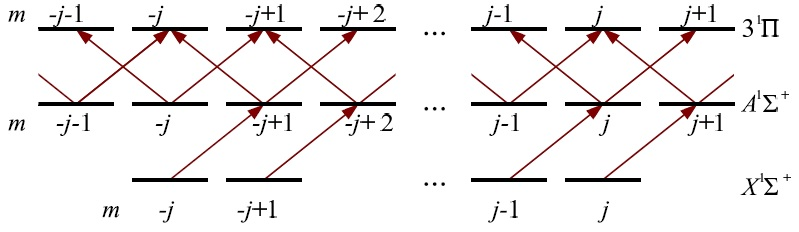
\includegraphics[width=0.9\textwidth]{m_potcurves.eps}
    \caption{Possible $m$ states and transitions: $3^1\Pi$ (top), $A^1\Sigma^+$ (middle), $X^1\Sigma^+$ (bottom)}
\label{fig:m_potcurves}
\end{figure}

The probe laser is linearly polarized; linear polarization can be expressed as
a superposition of left and right circularly polarized light.  Because of the
initial nonzero orientation of the system, the opposing circular polarizations
interact with the system differentially.  The left circular polarization will
see a different set of states that are available for transition than right
circular polarization.  After interacting with the sample, the remaining
superposition of both polarizations of light is passed through a linear
polarizer perpendicular to the initial polarization.  If the laser's total
polarization is unchanged, that is if transitions are not detected, no signal
will pass through the polarizer.  However, because the left and right circular
polarizations are absorbed differently, the superposition after interacting
with the system is no longer perfectly linear but rather elliptically
polarized.  Therefore, whatever signal is detected after the polarizer is
proportional to the final orientation~\cite{Jon15}.

\subsection{Previous Results}
A key feature of recent experimental results is the propensity for the change
in $j$ to be even numbers.  Recent theoretical calculations are in good
agreement with this result, as shown in Figure~\ref{fig:He_past_results}.  Note
that the theoretical rate constants were determined using the approximation that
the rate constant is proportional to the cross section times the average
velocity, as seen in Eq.~\ref{eq:rate_approx}.
\begin{equation}
    k\approx\sigma\overline v
\label{eq:rate_approx}
\end{equation}
\begin{figure}[ht]
    \centering
    \textbf{Helium Rate Constant}\par\medskip
    \includegraphics[width=0.7\textwidth]{He_past_results.eps}
    \caption{Experimental~\cite{Jon15} and theoretical~\cite{Mal15} rate constants}
\label{fig:He_past_results}
\end{figure}

It was originally thought that this propensity was related to the strict
selection rule for homonuclear diatomic molecules where no odd $\Delta j$
transitions are allowed at all.  Sodium and potassium are in the same column of
the periodic table, so it was thought that perhaps NaK was approximately
homonuclear, which would explain the propensity observed when the perturbing
atom is the noble gas helium or argon~\cite{Jon15}.  However, it has been
demonstrated that the propensity for an even $\Delta j$ depends on the
collision partner, whereas behavior of an approximately homonuclear molecule
should depend solely on the molecule.  Some experimental results for NaK in
certain states in a collision with potassium show no propensity for even
$\Delta j$ at all~\cite{Wol11}.  Unfortunately, theory has large computational
requirements, and it is computationally too expensive to model NaK+K to
confirm.  However, it can be concluded that some mechanism other than
approximate homonuclear behavior is affecting the $\Delta j$ propensity in both
experiment and theory.

\section{Analysis of Tipping Angle Distribution $B$}
\subsection{Goals: Physical Interpretations}
The large calculations for the theoretical analysis are used to calculate
$B_\lambda(j,j')$ values, which are the discrete probabilities for transferring
a specific amount of angular momentum ($\lambda$) to the NaK molecule in the
transition from $j$ to $j'$.  These calculations were done prior to the
beginning of the summer.

The goal of this summer's project was to gain a deeper physical understanding
of the angular momentum transitions.  The vector model facilitated
understanding the relationship between $\vectorize{j}$, $\vectorize{j'}$,
$\lambda$, and $\alpha$.  $\lambda$ gives the discrete value of angular
momentum transferred in the collision, or the distance between the tip of the
$\vectorize{j}$ vector and the tip of the $\vectorize{j'}$ vector in the vector
model.  Quantum mechanically, there are a finite number of discrete $\lambda$
values for a given $j\rightarrow j'$ transition.  $\alpha$ is the angle between
$\vectorize{j}$ and $\vectorize{j'}$ and is likewise discrete.

\subsection{Quantum Mechanical Model}
$B_\lambda(j,j')$ values are used to calculate the cross section of interaction; the
latter is given by Eq.~\ref{eq:QM_cross_section}.  $B_\lambda(j,j')$'s are discrete
probabilities for a particular transfer of angular momentum $\lambda$.
\begin{equation}
    \sigma(j\rightarrow j')=\frac{\pi}{(2j+1)k_j^2}{\sum_{\lambda=\lvert j-j'\rvert}^{j+j'} {(2\lambda+1)B_\lambda(j,j')}}
    \label{eq:QM_cross_section}
\end{equation}

$\lambda$ can best be described by extending the vector model to include two
different $\vectorize{j}$ vectors rather than one, such that $\vectorize{j}$ is the initial angular
momentum vector and $\vectorize{j'}$ is the final angular momentum vector.  See
Figure~\ref{fig:vectormodel_j_jp}.
\begin{figure}[ht!]
    \centering
    \includegraphics[width=0.5\textwidth]{vectormodel_j_jp_triangles.eps}
    \caption{$\lambda$'s relation to $\vectorize{j}$, $\vectorize{j'}$, and $\alpha$.}
\label{fig:vectormodel_j_jp}
\end{figure}
$\lambda$ is the distance between the tip of the $\vectorize{j}$ and $\vectorize{j'}$ vectors.  Since
$\vectorize{j}$ and $\vectorize{j'}$ can precess about the $z$ axis as well as have an altitude of any
allowed $\theta$, $\lambda$ can range in magnitude from the difference in the
two $\vectorize{j}$ vectors to their sum.  Physically, $\lambda$ represents how much
angular momentum was transferred in the collision.  The angle $\alpha$ is the
angle between $\vectorize{j}$ and $\vectorize{j'}$.  This parameter is called the tipping angle.  It is
a measure of how much the collision ``tipped'' $\vectorize{j'}$ from $\vectorize{j}$.

\subsection{Semiclassical Model}
In order to find a more intuitive physical interpretation, a semiclassical
model was used, based on ideas introduced by Derouard~\cite{Der84}.  Using the
law of cosines and the relationship shown in Figure~\ref{fig:vectormodel_j_jp},
the tipping angle can be related to the discrete amount of angular momentum, as
in Eq.~\ref{eq:loc_alpha_lambda}.  By allowing $\alpha$ to be a continuous
variable and making the appropriate substitutions, the discrete sum over
$\lambda$ in Eq.~\ref{eq:QM_cross_section} can be transformed to an integral
over $\alpha$, as in Eq.~\ref{eq:SC_cross_section}.
\begin{equation}
    \lambda(\lambda+1)=j(j+1)+j'(j'+1)-2\sqrt{j(j+1)j'(j'+1)}\cos\alpha
    \label{eq:loc_alpha_lambda}
\end{equation}
\begin{equation}
    \sigma(j\rightarrow j')=\frac{\pi(j'+1/2)}{k_j^2}{\int_{0}^{\pi}{B(j,j',\cos\alpha)\sin\alpha d\alpha}}
    \label{eq:SC_cross_section}
\end{equation}
$B(j,j',\cos\alpha)$ is related to $B_\lambda(j,j')$.  Rather than a
discrete probability, it is the continuous distribution of tipping angles.

\subsection{Results of $B$ analysis}
Plotting the $B_\lambda(j,j')$ and $B(j,j',\cos\alpha)$ values against the tipping angle
$\alpha$ shows which $\alpha$'s are most likely.  Larger $B$ values correspond to
a more likely tipping angle.  Plotting $B$ vs. $\alpha$ shows which tipping angles
are most likely.  As $B$ tends to be larger for smaller $\alpha$, the most
probable tipping angles are small.  Helium and argon display similar overall
behaviors.  Compare Figure~\ref{fig:He_B_1921} to Figure~\ref{fig:Ar_B_1921}.
\begin{figure}[ht!]
    \centering
    \begin{subfigure}{0.49\textwidth}
        \includegraphics[width=\linewidth]{He_Bplot_j19jp21.eps}
        \caption{Helium}
\label{fig:He_B_1921}
    \end{subfigure}
    \hspace*{\fill}
    \begin{subfigure}{0.49\textwidth}
        \includegraphics[width=\linewidth]{Ar_Bplot_j19jp21.eps}
        \caption{Argon}
\label{fig:Ar_B_1921}
    \end{subfigure}
    \caption{Comparison of discrete values $(2\lambda+1)B_\lambda(j,j')$ (shown as vertical lines) with the continuous function $B(j,j',\cos\alpha)$}
\label{fig:B_plots}
\end{figure}
\newline Both collisions favor small tipping angles.  Argon's $B$ values have
larger magnitudes than helium's $B$ values, so argon's cross sections also tend
to be larger.  Helium and argon tend to have similar rate constants, but argon
has lower average velocities at a given energy.  These trends are consistent
with Eq.~\ref{eq:rate_constants}.

\subsection{Conclusions for $B$ Analysis}
The quantum mechanical and semiclassical models agree rather well.  Both
exhibit oscillatory behavior as a function of angle, and the relative
magnitudes between peaks and troughs tend to have similar trends.  For
simplicity, the following conclusions apply to both models.

Helium's $B$ values were larger for even $\Delta j$ transitions than for odd
$\Delta j$ transitions, which was expected due to the propensity for even
$\Delta j$.  Argon showed no such propensity in its $B$ values.  This is not
entirely unexpected; in experiment, the propensity in collisions with helium is
much stronger than it is for argon.  Theoretical calculations successfully
demonstrate the propensity for helium, although the theoretical propensity is
much smaller than what has been observed in experiment.  It is possible that,
because argon's propensity is so much smaller than helium's, and because the
theoretical model attenuates the propensity with respect to experiment, the
propensity is too small for theory to detect at this point.  However, a refined
potential curve has recently been calculated~\cite{Pri15}, which may improve
the theoretical calculations.

As $\overline j$ increases, the expected tipping angle decreases.  As $\Delta
j$ increases, so does the average $\alpha$.  These conclusions for helium were
determined by treating even $\Delta j$ separately from odd $\Delta j$. For
example, as $\Delta j$ increases, the expected $\alpha$ for each successive
even $\Delta j$ is larger than the last. However, $\alpha$ for even $\Delta j$
tends to be smaller than for odd $\Delta j$ when the two $\Delta j$'s are not
far apart.

Overall, $\alpha$ tends to be small, especially for more likely transitions.
When the tipping angle is large, the transitions are less likely; likewise the
large tipping angles contribute less to the total number of transitions than
smaller tipping angles.

\section{Cross Section Analysis}
\subsection{$\Delta \theta$: Vector Model}
To analyze the cross sections, Eq.~\ref{eq:QM_cross_section}
and~\ref{eq:SC_cross_section} were evaluated as a sum over $\lambda$ for the
quantum mechanical model and as an integral over $\alpha$ for the semiclassical
model.  Finding the cross section averages over all possible collisions.
Recall the geometric relationship between $m$, $\vectorize{j}$, and $\theta$
from Eq.~\ref{eq:vector_model_geometry}.
\begin{equation*}
    \cos\theta=\frac{m}{\sqrt{j(j+1)}}
    \tag{\ref{eq:vector_model_geometry}}
\end{equation*}
$\Delta \theta$ is defined as:
\begin{equation}
    \Delta\theta\equiv\theta'-\theta
    \label{eq:delta_theta_def}
\end{equation}
Note that $\Delta\theta$ need not be the same as $\alpha$, the tipping angle.
Solving for $\theta$ from Eq.~\ref{eq:vector_model_geometry} and plugging it
into Eq.~\ref{eq:delta_theta_def} gives the relation in Eq.~\ref{eq:dtheta}.
\begin{equation}
    \Delta\theta = \arccos\left(\frac{m'}{\sqrt{j'(j'+1)}}\right)-\arccos\left(\frac{m}{\sqrt{j(j+1)}}\right)
    \label{eq:dtheta}
\end{equation}
The purpose of this analysis is to examine the cross sectional distribution
against $\Delta\theta$.  The difference between $\alpha$ and $\Delta\theta$
must not be overlooked.  $\alpha$ and $\Delta \theta$ are only equivalent if
$\vectorize{j}$ and $\vectorize{j'}$ are coplanar both with each other and the $z$ axis, as appears to
be the case in Figure~\ref{fig:vectormodel_coplanar}.
\begin{figure}[ht]
    \centering
    \begin{subfigure}{0.49\textwidth}
        \includegraphics[height=1\textwidth]{vectormodel_coplanar.eps}
        \caption{$\vectorize{j}$ and $\vectorize{j'}$ appear to be coplanar with each other and the $z$ axis, so $\alpha=\Delta\theta$}
\label{fig:vectormodel_coplanar}
    \end{subfigure}
    \hspace*{\fill}
    \begin{subfigure}{0.49\textwidth}
        \includegraphics[height=1\textwidth]{vectormodel_thetaprime_distribution.eps}
        \caption{Possible $\vectorize{j'}$ vectors given an initial $\vectorize{j}$ and $\alpha$}
\label{fig:vectormodel_tpdist}
    \end{subfigure}
    \caption{Vector model expansion}
\label{fig:vectormodelexpansion}
\end{figure}

It is much more common, however, for $\vectorize{j}$ and $\vectorize{j'}$ to precess about the $z$
axis.  For a particular $\alpha$ and initial $\theta$, then, the $\vectorize{j'}$ vector
can point anywhere on the circle in Figure~\ref{fig:vectormodel_tpdist}.

If the azimuthal angle $\phi$ in Figure~\ref{fig:vectormodel_tpdist} is a
continuous variable, there are exactly two possible $\vectorize{j'}$ vectors (and thus two
$\theta'$ values) where $\Delta\theta$ is exactly zero.  In this case,
$\vectorize{j}$ will not point in the same direction as $\vectorize{j'}$; $\vectorize{j}$ and $\vectorize{j'}$ will
never be collinear for a nonzero $\alpha$.

\subsection{Quantum Mechanical Analysis}
For the quantum mechanical model, $\Delta\theta$ was computed from the initial and final states
using $j$, $j'$, $m$, and $m'$ for all possible $m\rightarrow m'$ transitions,
as in Eq.~\ref{eq:dtheta}.  The cross sections associated with each
$\Delta\theta$ were put into a histogram using ranges of $\Delta\theta$.  A
convolution of the histogram values with a Gaussian transforms the discrete
probabilities into a distribution for comparison with the semiclassical model. This
process broadens the discrete values, which are essentially delta functions
($\delta\left(\Delta\theta\right)$), into a distribution that could be compared
with the semiclassical model.  Only a finite number of discrete values of $\phi$ (the
azimuthal angle in Figure~\ref{fig:vectormodel_tpdist}) are allowed due to
quantum mechanics. $\alpha$, $j$, $j'$, $m$, and $m'$ likewise have a finite
number of allowed values.

\subsection{Semiclassical Analysis}
The semiclassical model allows $\phi$ to be a continuous variable.  Given an initial
$\theta$, for all azimuthal $\phi$, a distribution of $\theta'$ can be
determined.  The final result is Eq.~\ref{eq:P_theta_thetaprime} which
represents the $\theta'$ distribution as a convolution of the tipping angle
distribution $B$.
\begin{equation}
    P(\theta,\theta')\sin\theta'=\frac{\sin\theta}{\pi}\int_{-1}^{1}\frac{B(j,j';\cos\theta\cos\theta'+y\sin\theta\sin\theta')}{\sqrt{1-y^2}}dy
    \label{eq:P_theta_thetaprime}
\end{equation}
A complete derivation can be found in Professor Hickman's work~\cite{Hic15},
but suffice it to say that the distribution integrates over all values of alpha
allowed by the geometry, and that the form is convenient for evaluation by
Gauss-Chebyshev quadrature of the first kind.  The range of integration is such
that $\cos\left(\theta+\theta'\right)<\cos\alpha<\cos\left(\theta-\theta'\right)$.

\subsection{Results: $\theta\rightarrow \theta'$}
The semiclassical distribution for a few chosen $\theta$ values can be seen in
Figure~\ref{fig:SC_t_tp}. For each distribution, the peak is centered where $\theta=\theta'$,
or, equivalently, where $\Delta\theta=0$.  The orientation tends to be
conserved, according to the semiclassical model.  The next section will show
that this result is also approximately valid quantum mechanically.
\begin{figure}[ht!]
    \centering
    \includegraphics[width=0.7\textwidth]{SC_theta_thetaprime_distribution_revised.eps}
    \caption{Distribution of $\theta'$ for $\theta=0^o$, $\theta=45^o$, $\theta=90^o$, $\theta=135^o$, $\theta=180^o$}
\label{fig:SC_t_tp}
\end{figure}

\subsection{Results: Cross Section vs. $\Delta\theta$} 
We averaged the quantum mechanical results over all possible $jm\rightarrow
j'm'$ transitions, calculating $\Delta\theta$ for each transition and weighting
each $\Delta\theta$ by the corresponding cross section.  This procedure enabled
us to construct the histogram as shown in Figure~\ref{fig:He_cs_jb30}, which
compares the semiclassical and quantum mechanical results for $j\rightarrow j'=28\rightarrow 32$.  The quantum mechanical
curve is difficult to see in this figure because the two models agree very
well.  However, the peak in the graph is evidently at $\Delta\theta=0$, which
is as expected.

As $\overline j$ increases, however, the agreement declines. The disagreement
depends both on the average value of $j$ and the value of $\Delta j$. It
appears that the smaller value of $j$ must not be too small.  When the smaller
value of $j$ is small, the disagreement is much greater.  As fewer $j$ states
can be averaged over, the behavior looks less classical and more quantum
mechanical.  See Figure~\ref{fig:He_cs_jb20_10}.
\begin{figure}[ht!]
    \centering
    \includegraphics[width=0.8\textwidth]{He_cs_jb30_dj4.eps}
    \caption{Cross sectional distribution vs. $\Delta\theta$, averaged over all collisions; $\overline j=30$}
\label{fig:He_cs_jb30}
\end{figure}
\begin{figure}[ht!]
    \centering
    \includegraphics[width=.49\textwidth]{He_cs_jb20_dj4.eps}
    \includegraphics[width=.49\textwidth]{He_cs_jb10_dj4.eps}
    \caption{Cross sectional distribution vs. $\Delta\theta$, averaged over all collisions; $\overline j = 20$ (left); $\overline j = 10$ (right)}
\label{fig:He_cs_jb20_10}
\end{figure}
For all $\overline j$, though, the most probable transitions are near small
$\Delta\theta$.  In the quantum mechanical model, however, the peak of the curve is rarely exactly
$\Delta\theta=0$.  Only a few transitions allow a $\Delta\theta$ of exactly 0.
This behavior is especially noticeable when $j$ and $j'$ are small or when
$\Delta j$ is very large.

\subsection{Results: $m\rightarrow m'$}
Filtering the quantum mechanical data by $m$ and $m'$ and smoothing with a spline gives
Figure~\ref{fig:He_cs_m_mp}.
\begin{figure}[ht!]
    \centering
    \includegraphics[width=0.8\textwidth]{QM_m_mprime_distribution.eps}
    \caption{Cross sectional distribution vs. $m'$ for the indicated initial quantum number $m$. Vertical lines represent where $\Delta m=0$} 
\label{fig:He_cs_m_mp}
\end{figure}
The curves do not all peak where $m=m'$, unlike
the $\theta\rightarrow\theta'$ distributions (Figure~\ref{fig:SC_t_tp}).  This
is to be expected.  $j$ and $j'$ change, and if $\theta$ is approximately
constant, then $m$ must change in such a way that $\Delta\theta$ is close to
zero.  Both the semiclassical and quantum mechanical models exhibit this behavior.  The semiclassical model does not
have the same oscillations that the quantum mechanical model has for $m\neq0$ curves, but it
appears to average over those oscillations, which is expected for a
semiclassical approximation to a quantum mechanical system.
\begin{figure}[ht!]
    \centering
    \includegraphics[width=0.8\textwidth]{SC_m_mprime_distribution.eps}
    \caption{Cross sectional distribution vs. $m'$ for the indicated initial quantum number $m$. The lines are the semiclassical calculations and the points are the quantum mechanical results.}
\label{fig:He_cs_m_mp_comp}
\end{figure}

\subsection{Conclusions for Cross Section Analysis}
Figure~\ref{fig:He_cs_m_mp_comp} illustrates the good agreement between semiclassical and
quantum mechanical calculations for $m\rightarrow m'$ transitions.  $\theta$ tends to be
conserved, which is consistent with other research in this field~\cite{Ale83}.
$m$ tends to change in such a way that $\Delta\theta$ is small.  This means the
orientation tends to be preserved during collisions of NaK with He and Ar.  The
physical interpretation of the vector model offers deeper understanding of this
behavior by modeling both $\vectorize{j}$ and $\vectorize{j'}$ vectors.  By
extending the vector model from one $\vectorize{j}$ vector to account for both
$j$ and $j'$, as well as modeling the changes in $m$ and $\theta$, it has been
shown that, for a particular $j$ to $j'$ transition, $m$ will change in a
certain way to approximately preserve $\theta$.  The semiclassical model is a
good approximation for the quantum mechanical model, especially when $j$ and
$j'$ are large.

\section{Acknowledgments}
A.C.T. acknowledges support by NSF under the REU program at Lehigh University
Physics Department and Grant Nos. PHY-0968898 and PHY-1403060.  Computational
facilities at the Texas Advanced Computing Center (TACC) used for this research
were supported by NSF from XSEDE resources provided by the XSEDE Science 
Gateways Program.  The author acknowledges stimulating conversations with J.
Huennekens, Teri Price, and Kara Richter as well as their patient hospitality.
The author would like to thank M. V. McSwain for logistical support.  The author
would like to thank A. P. Hickman for his explanations and mentorship.

\bibliography{allbib5}

\end{document}
